\documentclass[11pt]{article}

\usepackage{fullpage}
\usepackage{amsmath,amssymb,amsthm}
\usepackage{mathtools}
\usepackage{booktabs}
\usepackage{tikz}
\usetikzlibrary{arrows.meta,calc,decorations.pathreplacing,positioning}
\colorlet{okblue}{blue!55!black}
\colorlet{nored}{red!65!black}
\tikzset{
  slab/.style={fill=okblue,fill opacity=0.09,draw=none},
  slabedge/.style={okblue,line width=0.6pt},
  qpath/.style={line width=1.3pt,nored},
  ghost/.style={black!45,dash pattern=on 1pt off 1.6pt,line width=0.8pt},
  lbl/.style={font=\footnotesize}}
\setlength{\emergencystretch}{2em}
\setlength{\textfloatsep}{12pt}
\usepackage[colorlinks=true,linkcolor=blue,citecolor=blue,urlcolor=blue]{hyperref}
\usepackage[font={small,it}]{caption}

\theoremstyle{plain}
\newtheorem{theorem}{Theorem}[section]
\newtheorem{lemma}[theorem]{Lemma}
\newtheorem{proposition}[theorem]{Proposition}
\newtheorem{corollary}[theorem]{Corollary}
\theoremstyle{definition}
\newtheorem{definition}[theorem]{Definition}
\newtheorem{example}[theorem]{Example}
\theoremstyle{remark}
\newtheorem{remark}[theorem]{Remark}
\newtheorem{question}[theorem]{Open Problem}

\DeclareMathOperator{\tr}{tr}
\DeclareMathOperator{\Reg}{Reg}
\DeclareMathOperator{\spn}{span}
\DeclareMathOperator*{\argmax}{arg\,max}
\DeclareMathOperator*{\argmin}{arg\,min}
\newcommand{\R}{\mathbb{R}}
\newcommand{\E}{\mathbb{E}}
\newcommand{\Ball}{\mathbb{B}}
\newcommand{\wstar}{w^{\ast}}
\newcommand{\ip}[2]{\langle #1, #2\rangle}

\title{\vspace{-1.5cm}\bf Efficient Online Inverse Optimization with $O(\sqrt d)$ Regret}
\author{}
\date{}

\begin{document}
\maketitle
\vspace{-4em}

\begin{abstract}
We study online inverse linear optimization: each round, a learner recommends an action, then
observes the choice of an expert who maximizes a fixed, unknown linear criterion over $d$
attributes; the regret is the recommendations' total shortfall under that criterion. Bounds
polynomial in $d$ and uniform in the horizon are recent: $O(d)$ by Dewasurendra, by an improper
rule costing $T^{\Theta(d)}$ a round; $O(d)$ by Cai et al., by a deterministic proper rule costing
$O(d^{2})$; and the optimal order $O(\sqrt d)$ by Sakaue, in expectation, by a randomized improper
rule with no proved polynomial running time. We give a deterministic proper learner with regret at
most $\tfrac{51}{4}\sqrt d<13\sqrt d$ for every horizon, using one linear optimization and
$O(td^{2}+t^{2}d)$ arithmetic operations in round $t$, answering Sakaue's question on polynomial
time in the real-RAM model. The learner takes variable-metric steps whose rank-one stretches are
\emph{revocable}: a stretch stays active only while the query remains in a slab around the point
where it was made, and when it is revoked, the penalty it added to the query's distance from the
hidden criterion is refunded up to a term linear in the loss. The proof needs no randomization,
minimax theorem, knowledge set, projection or trace power.
\end{abstract}

\section{Introduction}\label{sec:intro}

Consider a resident who learns by watching the decisions of an attending physician on a hospital
ward. Every patient comes with a handful of possible interventions --- this drug or another, operate
now or wait --- and the attending picks one. The reasoning behind the pick is seldom spelled out: it
balances how well a treatment works against what it does to the patient, and how fast recovery
comes against what it costs. The resident never gets to see that balance, only its outcome, one
patient at a time. This is the problem of online inverse linear optimization.

We represent the attending's criterion by a fixed vector $\wstar$. Each intervention is a vector of
$d$ attributes, and the interventions available for the $t$-th patient form a set
$X_t\subseteq\R^{d}$. The resident proposes one, and is then shown the one the attending chose, a
maximizer of $\ip{\wstar}{\cdot}$ --- and nothing more: not the criterion, not what any option is
worth, not the size of the mistake. As in \cite{Cai26}, this leads to the following problem.

\smallskip
\noindent\textit{Online inverse linear optimization.} Fix a hidden $\wstar\in\Ball$. For
$t=1,2,\dots$:
\begin{enumerate}
\itemsep0pt \parskip0pt \topsep2pt
\item a compact nonempty action set $X_t\subseteq\Ball$ is revealed, chosen adversarially as a
      function of the history;
\item the learner recommends an action $\hat x_t\in X_t$;
\item the expert takes $x_t\in\argmax_{x\in X_t}\ip{\wstar}{x}$, which the learner then observes.
\end{enumerate}
\smallskip

Here $\Ball$ is the unit ball of $\R^{d}$ and $\|\cdot\|$ the Euclidean norm. The learner is charged
the cumulative shortfall of its recommendations, in the expert's own currency,
\begin{equation}\label{eq:regret}
  R_T\;:=\;\sum_{t=1}^{T}\ip{\wstar}{x_t-\hat x_t}\;\ge\;0 ,
\end{equation}
and never observes a single term of it. A bound is \emph{uniform in $T$} if it does not depend on
the horizon; it then bounds the total shortfall ever incurred. A learner is \emph{proper} if it
commits to an objective before it sees the menu: at the start of round $t$ it holds an estimate
$\hat w_t\neq0$ of $\wstar$ and recommends $\hat x_t\in\argmax_{x\in X_t}\ip{\hat w_t}{x}$, at the
cost of one linear optimization over $X_t$. It is \emph{improper} if $\hat x_t$ may be any function
of $X_t$ and the history. A proper learner carries an explicit hypothesis about the attending's
criterion, and each of its proposals is the best one under that hypothesis.

This paper is about the dimension. Bounds uniform in $T$ are now known (Table~\ref{tab:oilo}), so
the horizon is no longer the obstacle; what remains is how the total shortfall grows with $d$, the
number of attributes the criterion weighs. There is a floor: an adversary that offers the two
actions $\pm e_i$ in round $i\le d$ and draws the signs of $\wstar\in\{\pm1/\sqrt d\}^{d}$ at random
makes the better action of each round independent of everything seen before, so every learner,
even a randomized one, pays $\sqrt d$ in expectation \cite{SakaueONS,SakaueMMW}. We ask for a
learner that pays only that much and is also proper and \emph{efficient}, with
$\mathrm{poly}(d,T)$ arithmetic operations per round.

\begin{table}[t]
\centering\scriptsize\setlength{\tabcolsep}{4pt}
\begin{tabular}{@{}llllll@{}}
\toprule
Method & Regret & Uniform in $T$ & Proper & Deterministic & Per-round cost \\
\midrule
B\"armann et al.\ \cite{Barmann17,Barmann20} (OGD/MWU) & $O(\sqrt T)$ & no & yes & yes &
  $O(\tau_{\mathrm{sol}}+d)$ \\
Besbes et al.\ \cite{Besbes21,Besbes25} (circumcenter) & $O(d^{4}\ln T)$ & no & yes & yes &
  $\tau_{\mathrm{sol}}+\mathrm{poly}(d,T)$ \\
Gollapudi et al.\ \cite{GGKMPS} (centroid) & $O(d\ln T)$ & no & yes & yes &
  $\tau_{\mathrm{sol}}+\mathrm{poly}(d,T)$ \\
Gollapudi et al.\ \cite{GGKMPS} (John ellipsoid) & $\exp(O(d\ln d))$ & yes & yes & yes &
  $\tau_{\mathrm{sol}}+\mathrm{poly}(d,T)$ \\
Sakaue et al.\ \cite{SakaueONS} (online Newton step) & $O(d\ln T)$ & no & yes & yes &
  $O(\tau_{\mathrm{sol}}+d^{2}+\tau_{\mathrm{proj}})$ \\
Sakaue \cite{SakaueSOP} (second-order perceptron) & $O(d\ln T)$ & no & yes & yes &
  $O(\tau_{\mathrm{sol}}+d^{2})$ \\
Dewasurendra \cite{Dewasurendra26} (multiscale vote) & $O(d)$ & yes & no & yes & $T^{\Theta(d)}$ \\
Cai et al.\ \cite{Cai26} (variable metric) & $O(d)$ & yes & yes & yes &
  $O(\tau_{\mathrm{sol}}+d^{2})$ \\
Sakaue \cite{SakaueMMW} (multiscale matrix weights) & $O(\sqrt d)^{\dagger}$ & yes & no & no &
  $(dT)^{O(d)}\,\tau_{\mathrm{sol}}$ + finite \\
\midrule
\textbf{This paper} (revocable variable metric) & $\mathbf{O(\sqrt d)}$ & \textbf{yes} &
  \textbf{yes} & \textbf{yes} & $O(\tau_{\mathrm{sol}}+td^{2}+t^{2}d)$ \\
\quad with skipping (Prop.~\ref{prop:small}) & $\mathbf{O(\sqrt d)}$ & \textbf{yes} &
  \textbf{yes} & \textbf{yes} & amort.\ $O(\tau_{\mathrm{sol}}+d^{2}\log T)$ \\
\addlinespace
Lower bound \cite{SakaueONS}; \cite[Thm.~3.1]{Cai26} & $\Omega(\sqrt d)$ & --- & --- & --- & --- \\
\bottomrule
\end{tabular}
\caption{Regret $R_T$ of online inverse linear optimization on the unit ball. $\tau_{\mathrm{sol}}$:
one linear optimization over $X_t$; $\tau_{\mathrm{proj}}$: one Mahalanobis projection;
$^{\dagger}$in expectation.}
\label{tab:oilo}
\vspace{-1em}
\end{table}

\paragraph{History.} The online formulation is due to B\"armann, Pokutta and Schneider
\cite{Barmann17,Barmann20}, who obtained $O(\sqrt T)$ by online gradient descent and multiplicative
weights. Besbes, Fonseca and Lobel \cite{Besbes21,Besbes25} obtained $O(d^{4}\ln T)$ by a
circumcenter rule, ProjectedCones. Gollapudi, Guruganesh, Kollias, Manurangsi, Paes Leme and
Schneider \cite{GGKMPS}, who studied the same protocol as \emph{contextual recommendation},
obtained $O(d\ln T)$ by a centroid cutting-plane rule and $\exp(O(d\ln d))$, uniform in $T$, from
the John ellipsoid. Sakaue, Tsuchiya, Bao and Oki \cite{SakaueONS} obtained $O(d\ln T)$ at
$O(d^{2})$ per round plus a Mahalanobis projection by an online Newton step, together with the
lower bound above, and Sakaue \cite{SakaueSOP} kept $O(d\ln T)$ and removed the projection by a
second-order perceptron. Under structural assumptions the regret is finite: Sakaue, Bao and
Tsuchiya \cite{SakaueFY} assume that the gap in value of every action is at least a fixed multiple
of its distance to the optimal one, Oki and Sakaue \cite{OkiSakaue} that every $X_t$ is
$\mathrm{M}$-convex, as the bases of a matroid are, and Kitaoka \cite{Kitaoka26} obtains finite
regret and finitely many mistakes for the online Newton step on uniformly bounded integer action
sets, for $\wstar$ in the probability simplex and unique optimal actions; that bound carries a
factor $d^{2}$ and depends on the range of the coordinates. Whether a finite $\mathrm{poly}(d)$
bound holds for arbitrary action sets was asked in \cite{GGKMPS,OkiSakaue}. Dewasurendra
\cite{Dewasurendra26} answered it with $O(d)$, uniform in $T$: at every dyadic scale he covers the
class of optimality-gap functions, pools the resulting tolerant tests into one weighted vote and
plays the action the vote prefers --- an improper rule with $T^{\Theta(d)}$ tests per round. Cai,
Gupta, Gupta, Guruganesh, Jiang, Liaw, Mehta, Paes Leme, Velegkas and Wang \cite{Cai26} obtained
$O(d)$, precisely $\Reg_T\le6\sqrt3\,dR$ in the game below, with a deterministic proper rule at
$O(d^{2})$ per round: a variable-metric step with a self-normalized rank-one update, analyzed
through the trace power $\tr(H^{-1/2})$. Sakaue \cite{SakaueMMW} then reached the optimal order,
$\E[R_T]\le2^{21}\sqrt d$ for every $T$, without knowledge of $T$ and for arbitrary compact action
sets and ties, by matrix multiplicative weights on polynomial feature spaces at geometrically spaced
scales. The learner is randomized and improper --- it solves a linear program for a distribution
over a list of actions and samples from it --- and in round $t$ its finest scale acts on polynomials
of degree $\Theta(t^{4})$ in $d$ variables, with $(dT)^{O(d)}$ linear optimizations over $X_t$ in
its rational implementation.
Sakaue proves that every round terminates, gives no polynomial bound on the running time, and asks
whether $\sqrt d$ is attainable in time polynomial in the dimension, the horizon and the input
length \cite[Section~7]{SakaueMMW}. So far, then, $\sqrt d$ has been reached only by an
improper, randomized rule with no polynomial bound, and $O(d)$ is the best bound known for a proper
learner, for a deterministic one, and for an efficient one.

The problem is the online face of an older one --- recover an objective from observed optimal
decisions --- initiated by Burton and Toint \cite{BurtonToint} for shortest paths and cast in
linear-programming form by Ahuja and Orlin \cite{AhujaOrlin}; see \cite{ChanSurvey} for a survey.
Offline work turns on the choice of loss \cite{Keshavarz11,Bertsimas15,MohajerinEsfahani18,
Zattoni25}, on noisy \cite{Aswani18} or partially specified \cite{Ren25} data, and on statistical
rates \cite{Fatemi26}; applications run from control \cite{Akhtar21} and routing
\cite{ZattoniRouting} to offline reinforcement learning \cite{Dimanidis25}.

\paragraph{Reduction to a cutting-plane game.} As in \cite{Cai26}, we work with the following
primitive, isolated in \cite{GGKMPS}.

\smallskip
\noindent\textit{Cutting planes with a strong separation oracle.} A point $\wstar$ is hidden in a
known compact convex body $K_1\subseteq\R^{d}$; let $R:=\max_{w\in K_1}\|w\|>0$. For $t=1,2,\dots$:
\begin{enumerate}
\itemsep0pt \parskip0pt \topsep2pt
\item the learner queries a point $p_t\in\R^{d}$;
\item an adversary, having seen $p_t$ and the history, returns a unit vector $v_t$ subject only to
      $r_t:=\ip{\wstar-p_t}{v_t}\ge0$.
\end{enumerate}
The regret is $\Reg_T:=\sum_{t\le T}r_t$, a sum of nonnegative losses; the oracle is \emph{strong}
in that $v_t$ may be chosen after seeing $p_t$.
\smallskip

A learner for this game on $K_1=\Ball$ gives a proper learner for online inverse linear
optimization: play $\hat w_t:=p_t$ (any fixed nonzero vector if $p_t=0$), recommend
$\hat x_t\in\argmax_{x\in X_t}\ip{\hat w_t}{x}$, and return $v_t:=\delta_t/\|\delta_t\|$ for
$\delta_t:=x_t-\hat x_t$, skipping the rounds with $\delta_t=0$, which cost nothing. Optimality of
$\hat x_t$ and of $x_t$ gives $\ip{p_t}{\delta_t}\le0\le\ip{\wstar}{\delta_t}$, so
$r_t=\ip{\wstar-p_t}{\delta_t}/\|\delta_t\|\ge0$ and the round is legal, and as $\|\delta_t\|\le2$
the shortfall is $\ip{\wstar}{\delta_t}\le\ip{\wstar-p_t}{\delta_t}=\|\delta_t\|\,r_t\le2r_t$. Hence
$R_T\le2\Reg_T$; the expert need only be, round by round, at least as good as the recommendation
under its own criterion.

\subsection{Our Results}\label{sec:results}

We solve the cutting-plane game at the optimal rate, deterministically and in polynomial time.

Our main result is an algorithm which, given only the radius $R=\max_{w\in K_1}\|w\|$, has regret
$\Reg_T\le\tfrac{51}{8}R\sqrt d<6.4\,R\sqrt d$ for every horizon $T$, every hidden $\wstar\in K_1$
and every strong separation oracle, and whose round $t$ takes $O(td^{2}+t^{2}d)$ arithmetic
operations, $O(d^{2}+Td)$ per round on average over the first $T$ rounds
(Theorem~\ref{thm:rvm}). The bound is uniform in $T$, hence holds for $T=\infty$, and the algorithm
is deterministic and anytime: it needs neither $T$ nor restarts. Through the reduction above, with
$K_1=\Ball$, it gives a deterministic proper learner for online inverse linear optimization with
$R_T\le\tfrac{51}{4}\sqrt d<13\sqrt d$ for every horizon and every adaptive sequence of action sets,
using one linear optimization over $X_t$ and the same number of arithmetic operations per round
(Corollary~\ref{cor:oilo}).

Both bounds are optimal up to a constant factor: every learner, deterministic or randomized, suffers
$\Reg_d\ge\sqrt d\,R$ in the game on $K_1=R\Ball$ \cite[Theorem~3.1]{Cai26}, and $R_T\ge\sqrt d$ in
expectation for every $T\ge d$ \cite{SakaueONS,SakaueMMW}; our constants are within factors
$\tfrac{51}{8}<6.4$ and $\tfrac{51}{4}<13$ of these. Ours is the first $\sqrt d$ bound for online
inverse linear optimization that is deterministic, the first that is proper, and the first with a
polynomial bound on its computation, which answers the question of \cite{SakaueMMW} in the real-RAM
model, the model in which we count operations throughout. Our cost exceeds the $O(d^{2})$ of
\cite{Cai26} and grows with $t$. A variant that skips every stretch with $s_t^{2}\le(t+1)^{-4}$
keeps only $O(d\log t)$ stretches active, at an amortized $O(d^{2}\log T)$ arithmetic operations per
round and $O(d^{3}\log^{2}t)$ in the worst round, with regret below $6.41\,R\sqrt d$
(Proposition~\ref{prop:small}).

\paragraph{The algorithm.} Our starting point is the algorithm of \cite{Cai26}. From $p_1=0$ and
$H_1=I$ it updates
\begin{equation}\label{eq:vm}
  s_t=\|v_t\|_{H_t^{-1}},\qquad H_{t+1}=H_t+\frac{\tau}{s_t}\,v_tv_t^{\top},\qquad
  p_{t+1}=p_t+\alpha H_{t+1}^{-1}v_t ,
\end{equation}
with $\tau=\tfrac{1}{6d}$ and $\alpha=\tfrac{R}{2\sqrt3\,d}$, where $\|x\|_H:=(x^{\top}Hx)^{1/2}$.
It is a \emph{variable-metric} method: the positive definite matrix $H_t$ is a metric that records
what has been learned about $\wstar$, and each round \emph{stretches} it along the direction $v_t$
just received, to indicate that more is now known along $v_t$; the steps $H^{-1}v$ are then long in
directions not yet explored and short in explored ones. The analysis of \cite{Cai26} controls the
distance $\|p_t-\wstar\|_{H_t}$ in the current metric. Every stretch inflates that distance and is
never undone, which forces the stretches to stay small, $\tau=\Theta(1/d)$, and costs a factor
$\sqrt d$ over the lower bound.

We keep a metric, but a stretch is no longer permanent: it is \emph{revoked} as soon as the query
moves far, along its direction, from the query point at which it was made. The learner keeps a set
$A_t$ of \emph{active} stretches, and its metric is
\[
  H_t\;=\;I+\sum_{i\in A_t}\gamma_i\,v_iv_i^{\top} .
\]
Stretch $i$ is made at the end of round $i$, with a weight $\gamma_i$ and a \emph{slab} $L_i$, the
set of points strictly within $4\alpha s_i^{2}$ of $p_{i+1}$ along $v_i$, and it stays active only while the
query stays in $L_i$. In round $t$ the query moves continuously along $H^{-1}v_t$, for the metric
$H$ of the stretches still active, for a time $\alpha$; the moment it leaves the slab of an active
stretch, that stretch is revoked and the direction changes. At the end of the move a new stretch is
made. Formally, the algorithm is the following.

\begin{definition}[Algorithm RVM$(\alpha)$]\label{def:alg}
Fix $\alpha>0$. Start from $p_1=0$ and $A_1=\emptyset$. In round $t=1,2,\dots$, query $p_t$ and receive $v_t$. Then
follow the continuous path $\hat p_t:[0,\alpha]\to\R^{d}$ with right derivative given by
\begin{equation}\label{eq:move}
\begin{gathered}
  \hat p_t(0)=p_t,\qquad \hat p_t'(\eta)=\hat H_t(\eta)^{-1}v_t,\qquad
  \hat H_t(\eta)=I+\sum_{i\in\hat A_t(\eta)}\gamma_i\,v_iv_i^{\top},\\
  \hat A_t(\eta)=\bigl\{i\in A_t:\ \hat p_t(\tilde\eta)\in L_i\
    \text{for all}\ 0\le\tilde\eta\le\eta\bigr\},
\end{gathered}
\end{equation}
and set
\begin{equation}\label{eq:stretch}
\begin{gathered}
  p_{t+1}=\hat p_t(\alpha),\qquad s_t=\|v_t\|_{\hat H_t(\alpha)^{-1}},\qquad
  \gamma_t=\frac{1}{8s_t^{2}},\qquad
  L_t=\bigl\{p\in\R^{d}:\ |\ip{p-p_{t+1}}{v_t}|<4\alpha s_t^{2}\bigr\},\\
  A_{t+1}=\hat A_t(\alpha)\cup\{t\},\qquad H_{t+1}=\hat H_t(\alpha)+\gamma_t\,v_tv_t^{\top} .
\end{gathered}
\end{equation}
We run it with $\alpha=R/(3\sqrt d)$.
\end{definition}

The first display is the move and the second the stretch. In the move, $\hat A_t(\eta)$ is the set of
stretches whose slab the path has not yet left, so a stretch is revoked the moment the path reaches
the boundary of its slab, at $\eta=\alpha$ included, and never returns; without revocations the path
is a single segment and $p_{t+1}=p_t+\alpha H_t^{-1}v_t$, a variable-metric step like that of
\eqref{eq:vm}. By
Lemma~\ref{lem:wellposed} the path is well defined and piecewise linear, with at most $|A_t|+1$
pieces. The number $s_t\in(0,1]$ is the dual length of $v_t$ in the metric left after the move. The
weight makes $\gamma_ts_t^{2}=\tfrac18$, so by Sherman--Morrison the stretch lowers
$\|v_t\|^{2}_{H^{-1}}$ from $s_t^{2}$ to $\tfrac89s_t^{2}$: a constant-factor cut, as in the
ellipsoid method, but of the metric rather than of a feasible set. Compared with \eqref{eq:vm}, the
stretch has the same self-normalized form, with weight $\tau/s_t^{2}$ at the constant
$\tau=\tfrac18$ in place of $\tau/s_t$ at $\tau=\tfrac{1}{6d}$, and it comes with a slab that can
revoke it. The half-width $4\alpha s_t^{2}$ of $L_t$ is four times the largest distance
$\alpha s_t^{2}$ that the query can travel along $v_t$ in round $t$ (Lemma~\ref{lem:path}), and the
product $\gamma_t\cdot4\alpha s_t^{2}=\alpha/2$ of weight and half-width is the same for every
stretch; these two facts are what the analysis uses. Every quantity the update uses is observable
--- the queries, the directions received and the stretches made from them --- and neither the loss
$r_t$ nor $\wstar$ appears. The learner is proper, since its queries are its estimates, and uses no
randomness. Keeping $H^{-1}$ by Sherman--Morrison, round $t$ costs $O((k_t+1)(d^{2}+|A_t|d))$
operations, where $k_t$ is the number of stretches it revokes (Remark~\ref{rem:cost}); as
$|A_t|\le t-1$ and each stretch is revoked at most once, this gives the counts of
Theorem~\ref{thm:rvm}.

\begin{figure}[t]
\centering
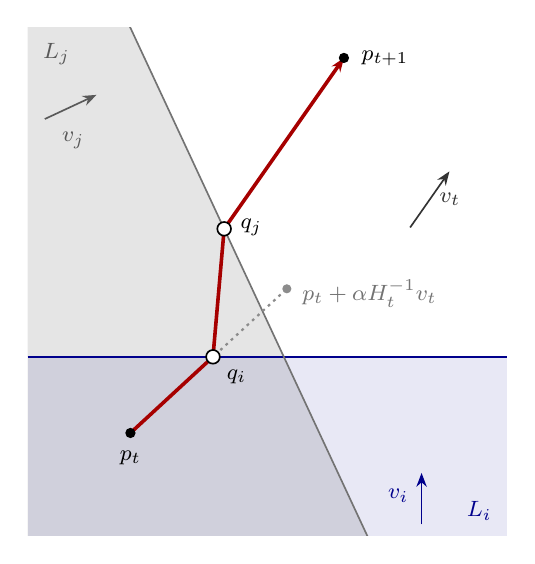
\begin{tikzpicture}[scale=1.45,>={Stealth[length=5pt]}]
  % alpha = 1, drawn at 8x. Stretch i: v_i = e_2, s_i^2 = 1/24 (gamma_i = 3, half-width 1/6).
  % Stretch j: v_j at 25 degrees, s_j^2 = 1/16 (gamma_j = 2, half-width 1/4). v_t at 55 degrees.
  \begin{scope}
    \clip (-0.9,-0.9) rectangle (3.3,3.55);
    \fill[black!10] ($(1.359,0.634)+10*(-0.4226,0.9063)$) -- ($(1.359,0.634)-10*(-0.4226,0.9063)$)
       -- ($(-2.265,-1.056)-10*(-0.4226,0.9063)$) -- ($(-2.265,-1.056)+10*(-0.4226,0.9063)$)
       -- cycle;
    \fill[slab] (-0.9,-2.0) rectangle (3.3,0.667);
    \draw[slabedge] (-0.9,0.667) -- (3.3,0.667);
    \draw[black!55,line width=0.6pt] (2.727,-2.3) -- (-0.024,3.6);
  \end{scope}
  \node[lbl,okblue,anchor=south east] at (3.25,-0.85) {$L_i$};
  \draw[->,okblue,line width=0.6pt] (2.55,-0.8) -- (2.55,-0.35);
  \node[lbl,okblue,anchor=east] at (2.52,-0.55) {$v_i$};
  \node[lbl,black!65,anchor=north west] at (-0.85,3.5) {$L_j$};
  \draw[->,black!65,line width=0.6pt] (-0.75,2.75) -- ($(-0.75,2.75)+(25:0.5)$);
  \node[lbl,black!65,anchor=north] at (-0.5,2.72) {$v_j$};
  \draw[->,black!80,line width=0.6pt] (2.45,1.8) -- ($(2.45,1.8)+(55:0.6)$);
  \node[lbl,black!80,anchor=west] at ($(2.45,1.8)+(55:0.3)$) {$v_t$};
  % the single step with the metric frozen
  \draw[ghost] (0,0) -- (1.370,1.263);
  \fill[black!45] (1.370,1.263) circle (0.04);
  \node[lbl,black!55,anchor=west] at (1.42,1.22) {$p_t+\alpha H_t^{-1}v_t$};
  % the path of the move
  \draw[qpath] (0,0) -- (0.723,0.667) -- (0.821,1.788);
  \draw[qpath,->] (0.821,1.788) -- (1.870,3.285);
  \fill (0,0) circle (0.045);
  \node[lbl,anchor=north] at (0,-0.07) {$p_t$};
  \draw[line width=0.6pt,fill=white] (0.723,0.667) circle (0.06);
  \node[lbl,anchor=north west] at (0.76,0.64) {$q_i$};
  \draw[line width=0.6pt,fill=white] (0.821,1.788) circle (0.06);
  \node[lbl,anchor=west] at (0.88,1.8) {$q_j$};
  \fill (1.870,3.285) circle (0.045);
  \node[lbl,anchor=west] at (1.94,3.285) {$p_{t+1}$};
\end{tikzpicture}
\caption{One move of RVM$(\alpha)$ in the plane, to scale ($\alpha=1$). The path (red) leaves the
slab $L_i$ at $q_i$ and the slab $L_j$ at $q_j$, turning at each revocation; the dotted segment is
the single step with the metric frozen.}
\label{fig:round}
\end{figure}

Figure~\ref{fig:round} gives the geometric picture. Two stretches $i$ and $j$ are active at $p_t$,
and each shortens the step along its own direction, so the path leaves $p_t$ bent away from $v_t$.
At $q_i$ it reaches the edge of $L_i$: stretch $i$ is revoked, the metric loses
$\gamma_iv_iv_i^{\top}$, and the path turns. At $q_j$ it leaves $L_j$, stretch $j$ is revoked too,
and the path continues along $v_t$ itself until time $\alpha$; stretch $t$ is then
made, with its slab centered at $p_{t+1}$ (its half-width $4\alpha s_t^{2}=4$ is off the picture).
The dotted segment is the single step $p_t+\alpha H_t^{-1}v_t$ with the metric frozen. It ends
outside both slabs, so revoking there would refund the two stretches at points beyond their
half-widths, which the analysis cannot afford (Remark~\ref{rem:why}). The slabs are not knowledge
sets: no point is ruled out, and $\wstar$ may lie anywhere.

% The three paragraphs below are switched off to keep the introduction to an idea of the
% algorithm. They predate the change of notation (c_t=p_{t+1}, B_t=4\alpha s_t^2, and the
% gaps a_t, b_t) and cite the removed Figure fig:ledger; update them before switching them on.
\iffalse
\paragraph{Why it works.} We track the squared distance to $\wstar$ in the metric in force,
\[
  \Phi\;=\;\|p-\wstar\|_{H}^{2}\;=\;\|p-\wstar\|^{2}+\sum_{i\in A}\gamma_i\ip{\wstar-p}{v_i}^{2} ,
\]
a Euclidean term plus, for each stretch in force, its weight times the squared gap to $\wstar$ along
its direction; $\Phi$ starts at $\|\wstar\|^{2}\le R^{2}$ and stays nonnegative. Between
revocations, the path of round $t$ lowers $\Phi$ at the rate
$2\ip{\wstar-p(\eta)}{v_t}=2(r_t-\xi(\eta))$, where $\xi(\eta)=\ip{p(\eta)-p_t}{v_t}$ is the
distance traveled along $v_t$. Revocations only shrink the metric, so
$0\le\xi(\eta)\le\eta s_t^{2}$, and the move changes $\Phi$ by at most
$-2\alpha r_t+\alpha^{2}s_t^{2}$ (Lemma~\ref{lem:path}). The jumps belong to the stretches. Making
stretch $t$ adds $\gamma_ta_t^{2}$, with $a_t=\ip{\wstar-c_t}{v_t}=r_t-\xi_t$ and
$\xi_t=\ip{p_{t+1}-p_t}{v_t}$; revoking it at a point $q_t$ removes $\gamma_tb_t^{2}$, with
$b_t=\ip{\wstar-q_t}{v_t}$. Writing $\Delta_t=\ip{q_t-c_t}{v_t}$, so that $|\Delta_t|\le B_t$
(Figure~\ref{fig:ledger}),
\[
  a_t^{2}-b_t^{2}\;=\;2\Delta_t\,r_t\;-\;\Delta_t(\Delta_t+2\xi_t) .
\]
The $r_t^{2}$ cancels: the penalty, quadratic in the loss, that a stretch charges when it is made is
refunded when it is revoked, up to a term linear in the loss, and $\gamma_tB_t=\alpha/2$ caps that
term by $\alpha r_t$, half of what the move of round $t$ earns. Over the lifetime of stretch $t$,
the move of round $t$ and the stretch together therefore contribute at most $-\alpha r_t$ if the
stretch is revoked, because then $|\Delta_t|=B_t$ and
$\gamma_t\Delta_t(\Delta_t+2\xi_t)\ge\gamma_tB_t(B_t-2\alpha s_t^{2})=\alpha^{2}s_t^{2}$ pays for
the move; and at most $-\alpha r_t+\tfrac98\alpha^{2}s_t^{2}$ if it survives to the end of round $T$,
with $q_t=p_{T+1}$ (Lemma~\ref{lem:lifetime}). In short, \emph{a revoked stretch pays for its own
step; a surviving one is paid for by the potential.} The potential is $\tr(\bar H^{-1})$, where
$\bar H$ is $I$ plus the surviving stretches, added one at a time in the order they were made
(Lemma~\ref{lem:potential}). It starts at $d$, stays nonnegative, and drops by at least $s_t^{2}/9$
at each surviving stretch $t$: the surviving stretches made earlier were in force throughout round
$t$, so $I$ plus their sum is dominated by $\hat H_t$, and $\gamma_ts_t^{2}=\tfrac18$. The surviving
stretches thus have $\sum s_t^{2}\le9d$, and
\[
  \alpha\,\Reg_T\;\le\;R^{2}+\frac98\,\alpha^{2}\cdot9d\;=\;R^{2}+\frac{81}{8}\,d\,\alpha^{2} ;
\]
at $\alpha=R/(3\sqrt d)$ this is $\Reg_T\le3R\sqrt d+\tfrac{27}{8}R\sqrt d=\tfrac{51}{8}R\sqrt d$.

\paragraph{Where the extra $\sqrt d$ went.} Nothing is revoked in \cite{Cai26}. There the stretch
inflates $D_t^{2}=\|p_t-\wstar\|_{H_t}^{2}$ by $\tfrac{\tau}{s_t}r_t^{2}\le\tau D_tr_t$
(Cauchy--Schwarz), which only the decrease $2\alpha r_t$ of the step can absorb. This forces
$\tau D_t\le\alpha$, hence $\tau\lesssim\alpha/R$ as $D_t$ can be of order $R$, and the budget
$\sum_ts_t^{2}\le4d/\tau$ then bounds the step term $\alpha\sum_ts_t^{2}$ only by $4d\alpha/\tau$,
at least of order $dR$ whatever $\alpha$ is. Revocation removes the constraint: the penalty
$\gamma_ta_t^{2}$ is never weighed against $\alpha r_t$ on its own, only the difference
$a_t^{2}-b_t^{2}$ is, and that is linear in $r_t$ with a coefficient bounded by the slab width. The
weight is then free to be $\tfrac{1}{8s_t^{2}}$ rather than $\tfrac{1}{6d\,s_t}$, the budget drops
from $24d^{2}$ to $9d$, and the step grows from $\alpha\sim R/d$ to $\alpha\sim R/\sqrt d$.

\paragraph{What the proof does not use.} Neither Klein's inequality nor a trace power: since
$\gamma_ts_t^{2}$ is the same for every stretch, the plain A-optimality criterion
$\tr(\bar H^{-1})$ of optimal design \cite{Kiefer74} does the work that $\tr(H^{-1/2})$ does in
\cite{Cai26}, and no $\log\det$ potential appears. The algorithm keeps no knowledge set or version
space, so it is not a cutting-plane method in the sense of \cite{NY,Vaidya,LSW}. It uses no
randomization, no linear program and no minimax theorem, and it projects nowhere: its iterates stay
within $1.46R$ of $\wstar$ on their own (Remark~\ref{rem:bounded}).
\fi

\paragraph{Organization.} Section~\ref{sec:analysis} states the results precisely and proves them.
After checking that the move is well defined and counting its cost, it bounds the change of
$\|p-\wstar\|_{H}^{2}$ over one move (Lemma~\ref{lem:path}), shows that over the lifetime of a stretch
its penalty is refunded up to a term linear in the loss (Lemma~\ref{lem:lifetime}), and pays for the
stretches that are never revoked with a trace potential (Lemma~\ref{lem:potential}).
Section~\ref{sec:further} shows why revocation is needed and why it happens exactly on the slab
boundary, and gives a variant with $O(d\log t)$ active stretches. Section~\ref{sec:open} concludes.

\section{Analysis}\label{sec:analysis}

We state the main results precisely and prove them. The first is the regret bound and cost of
RVM$(\alpha)$.

\begin{theorem}[Regret of RVM$(\alpha)$]\label{thm:rvm}
Let $R=\max_{w\in K_1}\|w\|$ and run RVM$(\alpha)$ with $\alpha=R/(3\sqrt d)$. Then for every $T$,
every $\wstar\in K_1$ and every strong separation oracle,
\[
  \Reg_T\;\le\;\frac{51}{8}\,R\sqrt d\;<\;6.4\,R\sqrt d
  \qquad\text{and}\qquad
  \|p_{T+1}-\wstar\|^{2}\;\le\;\frac{17}{8}\,R^{2} .
\]
Round $t$ uses $O(td^{2}+t^{2}d)$ arithmetic operations, and the first $T$ rounds use
$O(d^{2}+Td)$ per round on average.
\end{theorem}

Through the reduction of Section~\ref{sec:intro}, the theorem gives our result for online inverse
linear optimization.

\begin{corollary}[Online inverse optimization]\label{cor:oilo}
There is a deterministic proper learner for online inverse linear optimization with
\[
  R_T\;\le\;\frac{51}{4}\sqrt d\;<\;13\sqrt d
\]
for every $T$, every $\wstar\in\Ball$ and every adaptive sequence of action sets. Its round $t$
uses one linear optimization over $X_t$ and $O(td^{2}+t^{2}d)$ arithmetic operations, and its first
$T$ rounds use $O(d^{2}+Td)$ arithmetic operations per round on average.
\end{corollary}

\begin{proof}
Run RVM$(\alpha)$ on $K_1=\Ball$, so $R=1$, through the reduction of Section~\ref{sec:intro}, which
gives $R_T\le2\Reg_T$ and adds one linear optimization and $O(d)$ arithmetic operations per round,
one of them the square root that normalizes $v_t$. Rounds with $x_t=\hat x_t$ are not rounds of the
game, so the game's round index never exceeds $t$, and Theorem~\ref{thm:rvm} applies.
\end{proof}

The cost bounds of Theorem~\ref{thm:rvm} are counted in Remark~\ref{rem:cost}, once
Lemma~\ref{lem:wellposed} has checked that the move is well defined; the rest of the section proves
the regret bound.

The proof tracks the squared distance from the query to $\wstar$ in the metric in use,
$\|p-\wstar\|_{H}^{2}$ --- the quantity $\|p_t-\wstar\|_{H_t}^{2}$ of \cite{Cai26} --- through the
three kinds of events that change it: the moves, the making of stretches, and their revocation.
Lemma~\ref{lem:path} accounts for a move, \eqref{eq:ledger} regroups the whole run by stretch,
Lemma~\ref{lem:lifetime} bounds the contribution of each stretch over its lifetime, and
Lemma~\ref{lem:potential} bounds the total left over by the stretches that are never revoked.

\subsection{The move and its cost}\label{sec:wellposed}

The move \eqref{eq:move} defines the path and the set of active stretches in terms of each other.
The first lemma checks that exactly one path fits the definition and collects the facts about it
that the analysis uses.

\begin{lemma}[Well-posed move]\label{lem:wellposed}
In every round $t$ of RVM$(\alpha)$:
\begin{enumerate}
\itemsep0pt
\item[(a)] the slab of every active stretch contains the query: $p_t\in L_i$ for all $i\in A_t$, so
      that $\hat A_t(0)=A_t$ and $\hat H_t(0)=H_t$;
\item[(b)] exactly one path satisfies \eqref{eq:move}; it is piecewise linear with at most
      $k_t+1\le|A_t|+1$ pieces, where $k_t:=|A_t\setminus\hat A_t(\alpha)|$ is the number of
      stretches revoked in the round;
\item[(c)] $\hat H_t(\eta)$ is nonincreasing in $\eta$, so the dual length
      $\sigma(\eta):=\|v_t\|_{\hat H_t(\eta)^{-1}}$ is nondecreasing, and $0<\sigma(\eta)\le s_t\le1$;
\item[(d)] each stretch $i$ revoked in the round is revoked at a point $q_i$ of the path on the
      boundary of its slab: $|\ip{q_i-p_{i+1}}{v_i}|=4\alpha s_i^{2}$.
\end{enumerate}
\end{lemma}

\begin{proof}
We prove (a) by induction on $t$ and derive (b)--(d) along the way. At $t=1$ there are no stretches.
Suppose (a) holds at round $t$, and build the path piece by piece. Suppose it is determined on
$[0,\eta_j]$, and let $A^{j}$ be the set of stretches whose slab it has not left, all of whose slabs
contain $\hat p_t(\eta_j)$ (for $j=0$, $\eta_0=0$ and $A^{0}=A_t$ by (a)). As long as the active set
stays $A^{j}$, the right derivative is the constant $u_j=\hat H_t(\eta_j)^{-1}v_t$, so the path is
the segment $\hat p_t(\eta_j)+(\eta-\eta_j)u_j$; along it each displacement $\ip{\hat
p_t(\eta)-p_{i+1}}{v_i}$, $i\in A^{j}$, is affine in $\eta$, starts strictly inside $(-4\alpha
s_i^{2},4\alpha s_i^{2})$, and first reaches its boundary at some $\eta>\eta_j$, or never. The piece
ends at $\eta_{j+1}$, the least such $\eta$ or $\alpha$, whichever comes first; at $\eta_{j+1}$ the
stretches on the boundary leave $\hat A_t(\eta_{j+1})$, and the others are strictly inside their
slabs. No other path satisfies \eqref{eq:move}: one that agreed with this one on a largest interval
$[0,\eta']$, $\eta'<\alpha$, would keep the active set $\hat A_t(\eta')$ on some
$[\eta',\eta'+\epsilon)$, as the slabs are open, and so, being continuous with a constant right
derivative there, agree with it beyond $\eta'$. Every piece except the last revokes at least one
stretch, which gives (b) and (d); and the stretches still active at $\eta=\alpha$ are strictly
inside their slabs at $p_{t+1}$. The new stretch has $\ip{p_{t+1}-p_{t+1}}{v_t}=0$, so
$p_{t+1}\in L_t$, which proves (a) for round $t+1$. For (c), the set $\hat A_t(\eta)$ only loses
elements, and each loss subtracts a positive semidefinite $\gamma_iv_iv_i^{\top}$ from the metric;
inversion reverses the Loewner order, so $\hat H_t(\eta)^{-1}$ is nondecreasing and so is
$\sigma(\eta)^{2}=v_t^{\top}\hat H_t(\eta)^{-1}v_t$. Finally $\hat H_t(\eta)\succeq I$ gives
$0\prec\hat H_t(\eta)^{-1}\preceq I$, hence
$0<\sigma(\eta)\le\sigma(\alpha)=s_t\le\|v_t\|=1$.
\end{proof}

\begin{remark}[Cost]\label{rem:cost}
The algorithm stores $M=H^{-1}$ for the metric in use, and, for each active stretch $i$, the
vector $v_i$, the numbers $\gamma_i,s_i$ and the displacement $\phi_i=\ip{p-p_{i+1}}{v_i}$ of the
current point. On a piece of the path it computes $u=Mv_t$ in $O(d^{2})$ operations and
$\beta_i=\ip{v_i}{u}$ for every active stretch in $O(|A_t|d)$; the piece ends at the least of the
remaining time and the exit times $(4\alpha s_i^{2}-\operatorname{sign}(\beta_i)\phi_i)/|\beta_i|$
over $\beta_i\neq0$, after which $p$ and the $\phi_i$ are advanced in $O(d+|A_t|)$. Revoking
stretch $i$ is the Sherman--Morrison downdate
\[
  M\;\leftarrow\;M+\frac{\gamma_i}{1-\gamma_iv_i^{\top}Mv_i}\,Mv_iv_i^{\top}M ,
\]
whose denominator equals $1/(1+\gamma_iv_i^{\top}N^{-1}v_i)>0$ for $N=H-\gamma_iv_iv_i^{\top}\succeq
I$ the metric after the downdate; making stretch $t$ is the update
$M\leftarrow M-\tfrac{1}{9s_t^{2}}Mv_tv_t^{\top}M$, since $\gamma_t/(1+\gamma_ts_t^{2})=1/(9s_t^{2})$.
Each costs $O(d^{2})$. By Lemma~\ref{lem:wellposed}(b), round $t$ therefore costs
\[
  O\bigl((k_t+1)(d^{2}+|A_t|\,d)\bigr)\;=\;O\bigl(td^{2}+t^{2}d\bigr)
\]
arithmetic operations, as $k_t\le|A_t|\le t-1$. Since each stretch is revoked at most once,
$\sum_{t\le T}k_t\le T$, so the first $T$ rounds cost $O(Td^{2}+T^{2}d)$ in total, that is,
$O(d^{2}+Td)$ per round on average, with memory $O(d^{2}+Td)$. No random bits are used. Apart from
the constant $\alpha$, all operations are rational, because $s_t$ enters only through
$s_t^{2}=v_t^{\top}Mv_t$. The counts are in the real-RAM model.
\end{remark}

\subsection{One move}\label{sec:move}

Fix $T$, $\wstar$ and the oracle. In round $t$, $\xi(\eta):=\ip{\hat p_t(\eta)-p_t}{v_t}$ is the
distance the query has moved along $v_t$ by time $\eta$ of the path, and
$\xi_t:=\xi(\alpha)=\ip{p_{t+1}-p_t}{v_t}$. For the stretch made in round $t\le T$, we let $q_t$ be
the point at which it is revoked if that happens by the end of round $T$ and $q_t:=p_{T+1}$
otherwise, and we put
\[
  \Delta_t\;:=\;\ip{q_t-p_{t+1}}{v_t} ,
\]
its displacement along $v_t$ from the point where it was made. The stretches that are not revoked by
the end of round $T$ form the set $A_{T+1}$, and we call them \emph{surviving}. By
Lemma~\ref{lem:wellposed}(a) and (d),
\begin{equation}\label{eq:delta}
  |\Delta_t|\;=\;4\alpha s_t^{2}\ \ \text{if stretch $t$ is revoked},\qquad
  |\Delta_t|\;<\;4\alpha s_t^{2}\ \ \text{if it survives} .
\end{equation}

Along the path the query moves along $\hat H_t(\eta)^{-1}v_t$, which decreases the distance to
$\wstar$ at the rate $2\ip{\wstar-\hat p_t(\eta)}{v_t}$, and each revocation removes one term from
the metric. The lemma records the net effect, together with the fact that the query cannot move far
along $v_t$ in one round.

\begin{lemma}[One move]\label{lem:path}
In every round $t$, $0\le\xi_t\le\alpha s_t^{2}$, and
\[
  \|p_{t+1}-\wstar\|_{\hat H_t(\alpha)}^{2}-\|p_t-\wstar\|_{H_t}^{2}
  \;\le\;-2\alpha r_t+\alpha^{2}s_t^{2}
  -\sum_{i\in A_t\setminus\hat A_t(\alpha)}\gamma_i\ip{\wstar-q_i}{v_i}^{2} .
\]
\end{lemma}

\begin{proof}
On a piece of the path the metric $H=\hat H_t(\eta)$ is fixed and $\hat p_t'=H^{-1}v_t$, so
\[
  \frac{d}{d\eta}\,\|\hat p_t(\eta)-\wstar\|_{H}^{2}\;=\;2\ip{\hat p_t(\eta)-\wstar}{H\hat p_t'(\eta)}
  \;=\;-2\ip{\wstar-\hat p_t(\eta)}{v_t}\;=\;-2\bigl(r_t-\xi(\eta)\bigr) ,
\]
using $\ip{\wstar-\hat p_t(\eta)}{v_t}=\ip{\wstar-p_t}{v_t}-\ip{\hat p_t(\eta)-p_t}{v_t}$. Here
$\xi(0)=0$ and $\xi'(\eta)=\ip{\hat p_t'(\eta)}{v_t}=v_t^{\top}\hat H_t(\eta)^{-1}v_t=\sigma(\eta)^{2}
\in(0,s_t^{2}]$ by Lemma~\ref{lem:wellposed}(c), so $0\le\xi(\eta)\le\eta s_t^{2}$; at $\eta=\alpha$
this is the first claim. The rate of change is therefore at most $-2r_t+2\eta s_t^{2}$, and
integrating over $[0,\alpha]$ gives $-2\alpha r_t+\alpha^{2}s_t^{2}$. At the end of a piece, revoking
stretch $i$ at $q_i=\hat p_t(\eta)$ subtracts $\gamma_i\ip{\wstar-q_i}{v_i}^{2}$ from the squared
distance, which gives the last term.
\end{proof}

If no stretch is revoked, $\sigma(\eta)=s_t$ throughout and the lemma holds with equality: it is the
familiar expansion
$\|p_t+\alpha H_t^{-1}v_t-\wstar\|_{H_t}^{2}=\|p_t-\wstar\|_{H_t}^{2}-2\alpha r_t+\alpha^{2}s_t^{2}$.

\paragraph{The ledger.} Making stretch $t$ at $p_{t+1}$ adds $\gamma_t\ip{\wstar-p_{t+1}}{v_t}^{2}$
to the squared distance: $\|p_{t+1}-\wstar\|_{H_{t+1}}^{2}=\|p_{t+1}-\wstar\|_{\hat H_t(\alpha)}^{2}
+\gamma_t\ip{\wstar-p_{t+1}}{v_t}^{2}$. Add this to Lemma~\ref{lem:path} and sum over $t\le T$. Each
stretch revoked by the end of round $T$ is revoked exactly once, so its refund
$\gamma_t\ip{\wstar-q_t}{v_t}^{2}$ appears exactly once. The surviving stretches have $q_t=p_{T+1}$,
so $\|p_{T+1}-\wstar\|_{H_{T+1}}^{2}=\|p_{T+1}-\wstar\|^{2}+\sum_{t\in
A_{T+1}}\gamma_t\ip{\wstar-q_t}{v_t}^{2}$, and $p_1=0$, $H_1=I$ give
$\|p_1-\wstar\|_{H_1}^{2}=\|\wstar\|^{2}$. The penalty and the refund of stretch $t$ combine: since
$\ip{\wstar-p_{t+1}}{v_t}=r_t-\xi_t$ and $\ip{\wstar-q_t}{v_t}=r_t-\xi_t-\Delta_t$,
\[
  \ip{\wstar-p_{t+1}}{v_t}^{2}-\ip{\wstar-q_t}{v_t}^{2}
  \;=\;\Delta_t\bigl(2(r_t-\xi_t)-\Delta_t\bigr)\;=\;2\Delta_tr_t-\Delta_t(\Delta_t+2\xi_t) ,
\]
and the $r_t^{2}$ cancels. Collecting,
\begin{equation}\label{eq:ledger}
  \|p_{T+1}-\wstar\|^{2}-\|\wstar\|^{2}\;\le\;\sum_{t=1}^{T}\Lambda_t,\qquad
  \Lambda_t\;:=\;-2\alpha r_t+\alpha^{2}s_t^{2}
  +\gamma_t\bigl(2\Delta_tr_t-\Delta_t(\Delta_t+2\xi_t)\bigr) .
\end{equation}
We read $\Lambda_t$ as the \emph{lifetime contribution} of stretch $t$: the move that preceded it,
and the penalty $\gamma_t\ip{\wstar-p_{t+1}}{v_t}^{2}$ charged when the stretch was made, net of the
refund $\gamma_t\ip{\wstar-q_t}{v_t}^{2}$ collected when it is revoked --- or, for a surviving
stretch, still owed at the end.

\subsection{The lifetime of a stretch}\label{sec:lifetime}

In \cite{Cai26} the penalty for stretching the metric is never refunded, and it is quadratic in the
loss: $\tfrac{\tau}{s_t}r_t^{2}$ there, $\gamma_t\ip{\wstar-p_{t+1}}{v_t}^{2}=\gamma_t(r_t-\xi_t)^{2}$
here. The point of revocation is that the refund cancels the quadratic part exactly, as the ledger
shows, leaving in $\Lambda_t$ a term linear in $r_t$ whose coefficient the slab controls.

\begin{lemma}[Lifetime of a stretch]\label{lem:lifetime}
For every $t\le T$ (recall $r_t\ge0$),
\[
  \Lambda_t\;\le\;-\alpha r_t\ \ \text{if stretch $t$ is revoked},\qquad
  \Lambda_t\;\le\;-\alpha r_t+\tfrac98\,\alpha^{2}s_t^{2}\ \ \text{if it survives} .
\]
\end{lemma}

\begin{proof}
Group the terms of $\Lambda_t$ by their dependence on the loss:
\[
  \Lambda_t\;=\;\underbrace{-2\alpha r_t+2\gamma_t\Delta_tr_t}_{\text{linear in }r_t}
  \;+\;\underbrace{\alpha^{2}s_t^{2}-\gamma_t\Delta_t(\Delta_t+2\xi_t)}_{\text{free of }r_t} .
\]
\emph{The linear part.} By \eqref{eq:delta}, $|\Delta_t|\le4\alpha s_t^{2}$, and
$\gamma_t\cdot4\alpha s_t^{2}=\alpha/2$; as $r_t\ge0$, $2\gamma_t\Delta_tr_t\le\alpha r_t$, so the
linear part is at most $-\alpha r_t$.

\emph{The rest, for a revoked stretch.} Here $|\Delta_t|=4\alpha s_t^{2}$, and
$0\le\xi_t\le\alpha s_t^{2}$ by Lemma~\ref{lem:path}, so
\[
  \gamma_t\Delta_t(\Delta_t+2\xi_t)\;\ge\;\gamma_t|\Delta_t|\bigl(|\Delta_t|-2\xi_t\bigr)
  \;\ge\;\frac{1}{8s_t^{2}}\cdot4\alpha s_t^{2}\bigl(4\alpha s_t^{2}-2\alpha s_t^{2}\bigr)
  \;=\;\alpha^{2}s_t^{2} .
\]
\emph{The rest, for a surviving stretch.} Here we only use
$\Delta_t(\Delta_t+2\xi_t)=(\Delta_t+\xi_t)^{2}-\xi_t^{2}\ge-\xi_t^{2}$, so the rest is at most
$\alpha^{2}s_t^{2}+\gamma_t\xi_t^{2}\le\alpha^{2}s_t^{2}+\tfrac{1}{8s_t^{2}}\alpha^{2}s_t^{4}
=\tfrac98\alpha^{2}s_t^{2}$.
\end{proof}

The two cases say: \emph{a revoked stretch pays for its own step}, since leaving the slab takes the
query a distance $4\alpha s_t^{2}$ along $v_t$ and the refund on the way out covers the cost
$\alpha^{2}s_t^{2}$ of the move that preceded the stretch; a surviving stretch leaves its
$\tfrac98\alpha^{2}s_t^{2}$ to be paid by the potential of the next lemma. The constants in
\eqref{eq:stretch} are the ones that make the first case balance exactly: with weight
$\gamma_t=\tau/s_t^{2}$ and a half-width $h_t$ with $\gamma_th_t=\alpha/2$, the refund margin is
$\tfrac{\alpha}{2}(h_t-2\alpha s_t^{2})=\alpha^{2}s_t^{2}(\tfrac{1}{4\tau}-1)$, which covers
$\alpha^{2}s_t^{2}$ exactly when $\tau\le\tfrac18$.

\subsection{The surviving stretches}\label{sec:pot}

It remains to bound $\sum_{t\in A_{T+1}}s_t^{2}$. The metric in use is not monotone, since stretches
come and go, so we look instead at the metric built from the surviving stretches alone,
\[
  \bar H_t\;:=\;I+\sum_{i\in A_{T+1},\ i<t}\gamma_iv_iv_i^{\top}\qquad(t=1,\dots,T+1) ,
\]
which is monotone, and use the potential $\tr(\bar H_t^{-1})$: it starts at $d$ and never goes
negative.

\begin{lemma}[Surviving stretches]\label{lem:potential}
$\displaystyle\sum_{t\in A_{T+1}}s_t^{2}\;\le\;9\bigl(d-\tr(\bar H_{T+1}^{-1})\bigr)\;\le\;9d$.
\end{lemma}

\begin{proof}
If $t\notin A_{T+1}$ then $\bar H_{t+1}=\bar H_t$. Fix $t\in A_{T+1}$ and put
$\bar s_t:=\|v_t\|_{\bar H_t^{-1}}$. A surviving stretch $i<t$ was made before round $t$ and is never
revoked, so it is active throughout round $t$; hence $i\in\hat A_t(\alpha)$, so
$\bar H_t\preceq\hat H_t(\alpha)$, and inverting, $\bar s_t\ge s_t$. By Sherman--Morrison,
$\bar H_{t+1}^{-1}=\bar H_t^{-1}-\tfrac{\gamma_t}{1+\gamma_t\bar s_t^{2}}\bar H_t^{-1}v_tv_t^{\top}\bar
H_t^{-1}$, so
\[
  \tr(\bar H_t^{-1})-\tr(\bar H_{t+1}^{-1})
  \;=\;\frac{\gamma_t\,\|\bar H_t^{-1}v_t\|^{2}}{1+\gamma_t\bar s_t^{2}}
  \;\ge\;\frac{\gamma_t\,\bar s_t^{4}}{1+\gamma_t\bar s_t^{2}}
  \;\ge\;\frac{\bar s_t^{2}/8}{1+1/8}\;=\;\frac{\bar s_t^{2}}{9}\;\ge\;\frac{s_t^{2}}{9} .
\]
The first inequality is Cauchy--Schwarz, $\|\bar H_t^{-1}v_t\|\ge\ip{v_t}{\bar H_t^{-1}v_t}=\bar
s_t^{2}$ as $\|v_t\|=1$; the second holds because the middle expression is increasing in $\gamma_t$
and $\gamma_t=1/(8s_t^{2})\ge1/(8\bar s_t^{2})$. Telescoping from $\tr(\bar H_1^{-1})=d$ gives the
first bound, and $\tr(\bar H_{T+1}^{-1})>0$ the second.
\end{proof}

\begin{remark}[The potential]\label{rem:potential}
In optimal experimental design, a design is \emph{A-optimal} if it minimizes $\tr(H^{-1})$, where
$H$ is its information matrix: for least squares with homoscedastic noise, $H^{-1}$ is the
covariance of the estimate up to a constant, so the criterion is the average variance of the
estimated coordinates, ``A'' for average \cite{Kiefer74,Pukelsheim93}. The metric $\bar H_t$ has
the same form, each stretch adding $\gamma_iv_iv_i^{\top}$ as an observation along $v_i$ with weight
$\gamma_i$ adds to an information matrix, and the potential of Lemma~\ref{lem:potential} is this
criterion. The previous algorithm \cite{Cai26} needed the trace power $\tr(H^{-1/2})$ instead, and
the difference comes from the weight. There $\gamma_t=\tau/s_t$, and the computation above gives a
drop of order $\tau s_t^{3}$ only, too little to pay for $s_t^{2}$; the trace power, through Klein's
inequality, recovers $s_t^{2}$. Here $\gamma_t\bar s_t^{2}$ is at least a constant, so the drop in
$\tr(\bar H^{-1})$ is already of order $\bar s_t^{2}$.
\end{remark}

\subsection{Proof of Theorem~\ref{thm:rvm}}\label{sec:proof}

By \eqref{eq:ledger} and Lemma~\ref{lem:lifetime},
\[
  \|p_{T+1}-\wstar\|^{2}-\|\wstar\|^{2}\;\le\;-\alpha\sum_{t\le T}r_t
  +\frac98\,\alpha^{2}\!\!\sum_{t\in A_{T+1}}\!\!s_t^{2} ,
\]
and Lemma~\ref{lem:potential} bounds the last sum by $9d$. With $\|\wstar\|\le R$ and
$\alpha=R/(3\sqrt d)$, so that $d\alpha^{2}=R^{2}/9$,
\[
  \alpha\,\Reg_T+\|p_{T+1}-\wstar\|^{2}\;\le\;R^{2}+\frac{81}{8}\,d\alpha^{2}
  \;=\;R^{2}+\frac98R^{2}\;=\;\frac{17}{8}R^{2} .
\]
Both terms on the left are nonnegative. Dropping the second gives
$\Reg_T\le\tfrac{17}{8}R^{2}/\alpha=\tfrac{51}{8}R\sqrt d$, and dropping the first gives
$\|p_{T+1}-\wstar\|^{2}\le\tfrac{17}{8}R^{2}$. \qed

\medskip
The choice of $\alpha$ balances the two terms of $\Reg_T\le R^{2}/\alpha+\tfrac{81}{8}d\alpha$; the
exact minimizer $\alpha=\sqrt{8/81}\,R/\sqrt d$ improves $\tfrac{51}{8}=6.375$ only to
$\tfrac{9}{\sqrt2}\approx6.364$.

\section{Further Properties}\label{sec:further}

We explain why revocation is needed and why it happens exactly on the slab boundary, and give a
variant with $O(d\log t)$ active stretches.

% Switched off at the author's request.
\iffalse
\subsection{Bounded iterates}\label{sec:bounded}

\begin{remark}[No projection]\label{rem:bounded}
The update has no projection step, and needs none: Theorem~\ref{thm:rvm} bounds
$\|p_{T+1}-\wstar\|\le\sqrt{17/8}\,R<1.46\,R$ for every $T$, so every query satisfies
$\|p_t\|<2.46\,R$. The algorithm keeps no domain; the iterates stay bounded on their own, as in
\cite{Cai26,SakaueSOP}. The queries need not lie in $K_1$, which the game allows.
\end{remark}
\fi

\subsection{Why revocation, and why on the boundary}\label{sec:why}

\begin{remark}[Stalling without revocation]\label{rem:stall}
The weight $\gamma_t=1/(8s_t^{2})$ is far heavier than the weight $\tau/s_t$, $\tau=\tfrac{1}{6d}$,
of \cite{Cai26}, and without revocation it would stop the query. On $K_1=R\Ball$ take $\wstar=Re_1$
and let the oracle answer $v_t=e_1$ in every round, which is legal as long as $\ip{p_t}{e_1}\le R$.
If no stretch were ever revoked, the metric would be $\mathrm{diag}(\mu_t,1,\dots,1)$ with
$s_t^{2}=1/\mu_t$ and $\mu_{t+1}=\mu_t+\gamma_t=\tfrac98\mu_t$, so round $t$ would advance the query
along $e_1$ by $\alpha/\mu_t=\alpha(\tfrac89)^{t-1}$, and all rounds together by at most
$9\alpha=3R/\sqrt d$. For $d\ge10$ the query would never reach $\wstar$, and every round would lose
$r_t\ge R(1-3/\sqrt d)$. With revocation, a stretch stays active only until the query has
advanced $4\alpha s_i^{2}$ past $p_{i+1}$, the point where it was made, so a direction that keeps
being confirmed does not keep accumulating weight, and Theorem~\ref{thm:rvm} bounds the total loss
by $\tfrac{51}{8}R\sqrt d$.
\end{remark}

\begin{remark}[Revocation exactly on the boundary]\label{rem:why}
Lemma~\ref{lem:lifetime} uses \eqref{eq:delta} in both directions, and each fails under a simpler
rule. Without revocation every stretch survives and nothing bounds $\Delta_t$: the refund
$\gamma_t\ip{\wstar-q_t}{v_t}^{2}$ is collected only at the end, where it can be zero, and then
$\Lambda_t$ contains the penalty $\gamma_t(r_t-\xi_t)^{2}\approx r_t^{2}/(8s_t^{2})$, which no
multiple of $-\alpha r_t$ absorbs when $r_t$ is large compared with $\alpha s_t^{2}$;
Remark~\ref{rem:stall} shows that this is not an artifact of the proof. Revoking a stretch before
the query leaves its slab gives $|\Delta_t|<4\alpha s_t^{2}$, and the refund need no longer cover
the cost $\alpha^{2}s_t^{2}$ of the move. Revoking it after the query leaves, as a single step with
the metric frozen followed by a check would do (the dotted segment in Figure~\ref{fig:round}),
gives $|\Delta_t|>4\alpha s_t^{2}$, and the linear part
$2\gamma_t\Delta_tr_t$ is no longer bounded by $\alpha r_t$. Nor does the general bound keep the
overshoot of a single step within a constant multiple of the half-width: the step moves the query
along $v_i$ by $\alpha|v_i^{\top}H_t^{-1}v_t|$, which Cauchy--Schwarz bounds only by
$\alpha\|v_i\|_{H_t^{-1}}\|v_t\|_{H_t^{-1}}\le\sqrt8\,\alpha s_is_t$, using
$\|v_i\|^{2}_{H_t^{-1}}\le1/(1+\gamma_i)<8s_i^{2}$ for $i\in A_t$ and $\|v_t\|_{H_t^{-1}}\le s_t$
(Lemma~\ref{lem:wellposed}(c)), and this exceeds the half-width $4\alpha s_i^{2}$ of $L_i$ by the
factor $s_t/(\sqrt2\,s_i)$, which is unbounded. This is why the move is split at the slab
boundaries.
\end{remark}

\subsection{Fewer active stretches}\label{sec:small}

In RVM$(\alpha)$ every round makes a stretch, and up to $t-1$ of them can be active at round $t$,
which is where the factor $t$ in the cost of Remark~\ref{rem:cost} comes from. A stretch with a tiny
$s_t$ carries a tiny slab and a tiny step, and skipping it costs almost nothing.

\begin{proposition}[Skipping small stretches]\label{prop:small}
Modify RVM$(\alpha)$ so that stretch $t$ is made only if $s_t^{2}>(t+1)^{-4}$, and otherwise
$A_{t+1}=\hat A_t(\alpha)$ and $H_{t+1}=\hat H_t(\alpha)$. With $\alpha=R/(3\sqrt d)$, for every
$T$, $\wstar\in K_1$ and strong separation oracle,
\[
  \Reg_T\;\le\;\Bigl(\frac{51}{8}+\frac{0.03}{d}\Bigr)R\sqrt d\;<\;6.41\,R\sqrt d ,
  \qquad
  |A_t|\;\le\;\frac{d\,\ln\bigl(1+t^{5}/(8d)\bigr)}{\ln(9/8)}\;=\;O(d\log t)\quad\text{for all }t .
\]
Round $t$ then costs $O(d^{3}\log^{2}t)$ arithmetic operations, and the first $T$ rounds cost
$O(Td^{2}\log T)$ in total.
\end{proposition}

\begin{proof}
\emph{Regret.} Lemmas~\ref{lem:wellposed} and~\ref{lem:path} do not refer to the rule for making
stretches, and neither do Lemmas~\ref{lem:lifetime} and~\ref{lem:potential}, which concern stretches
that are made. In the ledger \eqref{eq:ledger}, a round that makes no stretch contributes
$\Lambda_t=-2\alpha r_t+\alpha^{2}s_t^{2}\le-\alpha r_t+\alpha^{2}(t+1)^{-4}$, as
$s_t^{2}\le(t+1)^{-4}$. The proof of Theorem~\ref{thm:rvm} then gives
$\alpha\Reg_T\le\tfrac{17}{8}R^{2}+\alpha^{2}\sum_{t\ge1}(t+1)^{-4}$, and
$\sum_{n\ge2}n^{-4}=\tfrac{\pi^{4}}{90}-1<0.083$, so
$\Reg_T\le\tfrac{51}{8}R\sqrt d+0.083\,\alpha\le\tfrac{51}{8}R\sqrt d+0.028\,R/\sqrt d$.

\emph{Active stretches.} Fix $t$ and list $A_t=\{i_1<\dots<i_k\}$. Put $G_1=I$ and
$G_{j+1}=G_j+\gamma_{i_j}v_{i_j}v_{i_j}^{\top}$, so that $G_{k+1}=H_t$. Each $i_l$ with $l<j$ was made
before round $i_j$ and is still active at round $t$, so it was active throughout round $i_j$;
hence $G_j\preceq\hat H_{i_j}(\alpha)$ and $v_{i_j}^{\top}G_j^{-1}v_{i_j}\ge s_{i_j}^{2}$. By the matrix
determinant lemma and $\gamma_is_i^{2}=\tfrac18$,
\[
  \det H_t\;=\;\prod_{j=1}^{k}\bigl(1+\gamma_{i_j}v_{i_j}^{\top}G_j^{-1}v_{i_j}\bigr)
  \;\ge\;\Bigl(\frac98\Bigr)^{k} .
\]
On the other hand every stretch made has $\gamma_i=1/(8s_i^{2})<(i+1)^{4}/8$, so
$\tr H_t\le d+\tfrac18\sum_{i=1}^{t-1}(i+1)^{4}\le d+t^{5}/8$, and the inequality of arithmetic and
geometric means gives $\det H_t\le(\tr H_t/d)^{d}\le(1+t^{5}/(8d))^{d}$. Comparing the two bounds
gives the claim on $|A_t|$.

\emph{Cost.} By Remark~\ref{rem:cost}, a piece costs $O(d^{2}+|A_t|d)=O(d^{2}\log t)$, round $t$ has
at most $|A_t|+1$ pieces, and the first $T$ rounds have at most $2T$ pieces in total.
\end{proof}

\section{Concluding Remarks}\label{sec:open}

We gave a deterministic proper learner for online inverse linear optimization with regret
$O(\sqrt d)$, the optimal order, using $\mathrm{poly}(d,T)$ arithmetic operations per round. It is
the variable-metric method of \cite{Cai26} with one change: stretches are revoked when the query
leaves their slab, which lets their weight be a constant multiple of $1/s_t^{2}$. The running time
still depends on $T$: the variant of Proposition~\ref{prop:small} takes $O(d^{2}\log T)$ operations
per round on average, the logarithm being the number of active stretches, whereas \cite{Cai26}
takes $O(d^{2})$ but has regret $O(dR)$. Whether regret $O(R\sqrt d)$ is possible with
$\mathrm{poly}(d)$ operations per round, independent of $T$, remains open. Also open is whether
$O(R\sqrt d)$ regret holds with polynomial bit complexity when quantities are rounded to
$\mathrm{poly}(d,\log T)$ bits, as our operation counts are in the real-RAM model and do not bound
the bit length of the weights $\gamma_t=1/(8s_t^{2})$ or of the entries of $H_t^{-1}$.

\paragraph{Formal verification.} The accompanying Lean~4 / Mathlib development machine-checks
Definition~\ref{def:alg}, Theorem~\ref{thm:rvm} (regret, iterate bound, and per-round/cumulative
instrumented scalar-operation bounds), Corollary~\ref{cor:oilo} (the protocol reduction, the full
chain $R_T\le2\Reg\le\tfrac{51}{4}\sqrt d<13\sqrt d$, existence of best actions over nonempty
compact action sets, the explicitly constructed closed-loop deterministic proper learner carrying
the incremental Sherman--Morrison state with tie-round skipping, and its own per-round/cumulative
scalar-operation bounds), Lemma~\ref{lem:wellposed} (including existence, uniqueness, continuity,
and piecewise linearity of the path), Remark~\ref{rem:cost} (combinatorial piece and revocation
bounds, Sherman--Morrison update/downdate identities, exact state equivalence of the incremental
matrix-inversion-free implementation storing $s_t^2$ with purely rational arithmetic and active
displacements on $A_t$, and per-round scalar-operation bounds), Lemma~\ref{lem:path},
\eqref{eq:ledger}, Lemma~\ref{lem:lifetime}, Lemma~\ref{lem:potential}, Remark~\ref{rem:stall}
(tied to the explicit algorithm without revocation), and Proposition~\ref{prop:small} (regret,
determinant/trace/$|A_t|$ bounds, full state equivalence of the incremental skipping
implementation, and per-round/cumulative scalar-operation bounds), using only the standard
classical axioms (\texttt{propext}, \texttt{Classical.choice}, \texttt{Quot.sound}). The
operation-count model (\texttt{CostM}, with a private constructor and \texttt{CostM.foldl} loops)
tracks instrumented scalar-operation counts of the incremental implementation, charging $1$
operation per scalar arithmetic or comparison primitive; index and finite-set bookkeeping, memory
operations (including the $O(d^2+Td)$ memory bound), bit-level rationality, and the internal cost
of the linear-optimization oracle over $X_t$ in Corollary~\ref{cor:oilo} are not charged. Rounds in
the Lean development are $0$-indexed ($t=0,1,\dots$), corresponding to round $t+1$ in this paper.
The weaker-expert remark in Section~\ref{sec:intro}, the prose remarks after Lemmas~\ref{lem:path}
and~\ref{lem:lifetime} and Theorem~\ref{thm:rvm}, the informal discussion in
Remarks~\ref{rem:potential} and~\ref{rem:why}, and the cited lower bounds are not formalized.

% Open problems switched off at the author's request.
\iffalse
\begin{question}[Bit complexity]\label{op:bits}
Does RVM$(\alpha)$ with every quantity rounded to $\mathrm{poly}(d,\log T)$ bits keep regret
$O(R\sqrt d)$? Sakaue \cite{SakaueMMW} asks for running time polynomial in $d$, $T$ and the input
length, and our counts are in the real-RAM model. The operations of RVM$(\alpha)$ are rational apart
from $\alpha$, and the reduction adds one square root per round, but nothing in our analysis bounds
the weights $\gamma_t=1/(8s_t^{2})$ or the bit length of the entries of $H_t^{-1}$.
Lemma~\ref{lem:lifetime} would survive slabs that are left only approximately, since it uses
\eqref{eq:delta} only up to constant factors; the harder part is Lemma~\ref{lem:path}, whose proof
relies on the velocity being exactly $H^{-1}v_t$ for the metric $H$ in use.
\end{question}

\begin{question}[The constant]\label{op:constant}
What is the value of the game? The upper bound is $\tfrac{51}{8}R\sqrt d$ and the lower bound $\sqrt
d\,R$, and when the loss $r_t$ is revealed the value is exactly $\sqrt d\,R$
\cite[Proposition~3.3]{Cai26}. In our proof, half of the decrease $-2\alpha r_t$ is spent on the
linear part of the refund (weight times half-width is $\gamma_t\cdot4\alpha s_t^{2}=\alpha/2$), the
revoked stretches force $\tau\le\tfrac18$ in $\gamma_t=\tau/s_t^{2}$, and the potential then charges
$(1+\tau)/\tau=9$ per unit of $s_t^{2}$. With half-width $\kappa\alpha s_t^{2}/\tau$ in place of
$4\alpha s_t^{2}$, so that weight times half-width is $\kappa\alpha$, the same argument allows
$\tau\le\kappa^{2}/(1+2\kappa)$ and yields the constant
$(1+\kappa)^{2}/(\kappa(1-\kappa)\sqrt{1+2\kappa})$ at the best $\alpha$, which is least, about
$6.09$, near $\kappa=0.4$: trading the three losses against one another gains little, and anything
close to $1$ needs a different argument.
\end{question}
\fi

\begin{thebibliography}{99}

\bibitem{AhujaOrlin}
R.~K.~Ahuja and J.~B.~Orlin,
\emph{Inverse Optimization},
Oper.\ Res.\ 49(5):771--783, 2001.

\bibitem{Akhtar21}
S.~A.~Akhtar, A.~S.~Kolarijani and P.~Mohajerin Esfahani,
\emph{Learning for Control: An Inverse Optimization Approach},
IEEE Control Syst.\ Lett.\ 6:187--192, 2021.

\bibitem{Aswani18}
A.~Aswani, Z.-J.~Shen and A.~Siddiq,
\emph{Inverse Optimization with Noisy Data},
Oper.\ Res.\ 66(3):870--892, 2018.

\bibitem{Barmann17}
A.~B\"armann, S.~Pokutta and O.~Schneider,
\emph{Emulating the Expert: Inverse Optimization through Online Learning},
ICML 2017, PMLR 70:400--410.

\bibitem{Barmann20}
A.~B\"armann, A.~Martin, S.~Pokutta and O.~Schneider,
\emph{An Online-Learning Approach to Inverse Optimization},
\texttt{arXiv:1810.12997}, 2020.

\bibitem{Bertsimas15}
D.~Bertsimas, V.~Gupta and I.~C.~Paschalidis,
\emph{Data-Driven Estimation in Equilibrium Using Inverse Optimization},
Math.\ Program.\ 153(2):595--633, 2015.

\bibitem{Besbes21}
O.~Besbes, Y.~Fonseca and I.~Lobel,
\emph{Online Learning from Optimal Actions},
COLT 2021, PMLR 134:586.

\bibitem{Besbes25}
O.~Besbes, Y.~Fonseca and I.~Lobel,
\emph{Contextual Inverse Optimization: Offline and Online Learning},
Oper.\ Res.\ 73(1):424--443, 2025.

\bibitem{BurtonToint}
D.~Burton and Ph.~L.~Toint,
\emph{On an Instance of the Inverse Shortest Paths Problem},
Math.\ Program.\ 53:45--61, 1992.

\bibitem{Cai26}
Y.~Cai, A.~Gupta, V.~Gupta, G.~Guruganesh, Y.~Jiang, C.~Liaw, A.~Mehta, R.~Paes Leme, G.~Velegkas
and D.~Wang,
\emph{Efficient Online Inverse Optimization with $O(d)$ Regret},
\texttt{arXiv:2609.13440}, 2026.

\bibitem{ChanSurvey}
T.~C.~Y.~Chan, R.~Mahmood and I.~Y.~Zhu,
\emph{Inverse Optimization: Theory and Applications},
Oper.\ Res.\ 73(2):1046--1074, 2025.

\bibitem{Dewasurendra26}
P.~Dewasurendra,
\emph{Multiscale Reward Hedging from Correct Demonstrations},
\texttt{arXiv:2608.06825}, 2026.

\bibitem{Dimanidis25}
I.~Dimanidis, T.~Ok and P.~Mohajerin Esfahani,
\emph{Offline Reinforcement Learning via Inverse Optimization},
\texttt{arXiv:2502.20030}, 2025.

\bibitem{Fatemi26}
P.~Fatemi, H.~Maskan, S.~Sra and P.~Mohajerin Esfahani,
\emph{Tight Generalization Bounds for Noiseless Inverse Optimization},
\texttt{arXiv:2605.08866}, 2026.

\bibitem{GGKMPS}
S.~Gollapudi, G.~Guruganesh, K.~Kollias, P.~Manurangsi, R.~Paes Leme and J.~Schneider,
\emph{Contextual Recommendations and Low-Regret Cutting-Plane Algorithms},
NeurIPS 2021; \texttt{arXiv:2106.04819}.

\bibitem{Keshavarz11}
A.~Keshavarz, Y.~Wang and S.~Boyd,
\emph{Imputing a Convex Objective Function},
IEEE Int.\ Symp.\ Intelligent Control, 2011, 613--619.

\bibitem{Kiefer74}
J.~Kiefer,
\emph{General Equivalence Theory for Optimum Designs (Approximate Theory)},
Ann.\ Statist.\ 2(5):849--879, 1974.

\bibitem{Kitaoka26}
A.~Kitaoka,
\emph{Online Inverse Integer Linear Optimization via Small-Gradient Skipping: Constant Regret and
Finite Mistakes},
\texttt{arXiv:2609.09809}, 2026.

\bibitem{LSW}
Y.~T.~Lee, A.~Sidford and S.~C.-W.~Wong,
\emph{A Faster Cutting Plane Method and its Implications for Combinatorial and Convex Optimization},
FOCS 2015, 1049--1065.

\bibitem{MohajerinEsfahani18}
P.~Mohajerin Esfahani, S.~Shafieezadeh-Abadeh, G.~A.~Hanasusanto and D.~Kuhn,
\emph{Data-Driven Inverse Optimization with Imperfect Information},
Math.\ Program.\ 167(1):191--234, 2018.

\bibitem{NY}
A.~S.~Nemirovski and D.~B.~Yudin,
\emph{Problem Complexity and Method Efficiency in Optimization},
Wiley, 1993.

\bibitem{OkiSakaue}
T.~Oki and S.~Sakaue,
\emph{Finite and Corruption-Robust Regret Bounds in Online Inverse Linear Optimization under
$\mathrm{M}$-Convex Action Sets},
ICML 2026; \texttt{arXiv:2602.01682}.

\bibitem{Pukelsheim93}
F.~Pukelsheim,
\emph{Optimal Design of Experiments},
Wiley, 1993; reprinted as SIAM Classics Appl.\ Math.\ 50, 2006.

\bibitem{Ren25}
K.~Ren, P.~Mohajerin Esfahani and A.~Georghiou,
\emph{Inverse Optimization via Learning Feasible Regions},
\texttt{arXiv:2505.15025}, 2025.

\bibitem{SakaueFY}
S.~Sakaue, H.~Bao and T.~Tsuchiya,
\emph{Revisiting Online Learning Approach to Inverse Linear Optimization: A Fenchel--Young Loss
Perspective and Gap-Dependent Regret Analysis},
AISTATS 2025, PMLR 258:46--54.

\bibitem{SakaueMMW}
S.~Sakaue,
\emph{Tight Regret Bound for Online Inverse Linear Optimization via Multiscale Matrix Weights},
\texttt{arXiv:2609.26978}, 2026.

\bibitem{SakaueONS}
S.~Sakaue, T.~Tsuchiya, H.~Bao and T.~Oki,
\emph{Online Inverse Linear Optimization: Efficient Logarithmic-Regret Algorithm, Robustness to
Suboptimality, and Lower Bound},
NeurIPS 2025; \texttt{arXiv:2501.14349}.

\bibitem{SakaueSOP}
S.~Sakaue,
\emph{Simple Projection-Free Algorithm for Contextual Recommendation with Logarithmic Regret and
Robustness},
\texttt{arXiv:2603.20826}, 2026.

\bibitem{Vaidya}
P.~M.~Vaidya,
\emph{A New Algorithm for Minimizing Convex Functions over Convex Sets},
Math.\ Program.\ 73:291--341, 1996.

\bibitem{Zattoni25}
P.~Zattoni Scroccaro, B.~Atasoy and P.~Mohajerin Esfahani,
\emph{Learning in Inverse Optimization: Incenter Cost, Augmented Suboptimality Loss, and
Algorithms},
Oper.\ Res.\ 73(5):2661--2679, 2025.

\bibitem{ZattoniRouting}
P.~Zattoni Scroccaro, P.~van Beek, P.~Mohajerin Esfahani and B.~Atasoy,
\emph{Inverse Optimization for Routing Problems},
Transportation Sci.\ 59(2):301--321, 2025.

\end{thebibliography}

\end{document}
